%%%%%%%%%%%%%%%%%%%%%%%%%%%%%%%%%%%%%%%%%%%%%%%%%%%%%%%%%%%%%%%%%%%%%%%%%%%
% Aclaraciones previas de compilación
%%%%%%%%%%%%%%%%%%%%%%%%%%%%%%%%%%%%%%%%%%%%%%%%%%%%%%%%%%%%%%%%%%%%%%%%%%%

% Esta es la versión para compilar cada clase por separado.
% Configurar la compilación rápida como LaTex + Bib(la)tex + LaTeX(x2) + dvips+ pvs2pdf + ver pdf
% En caso de precisar agregar un paquete, agregarlo a paquetes.tex
% Para limpiar de archivos auxiliares la copia local del repositorio correr bash remove-aux-files.sh

%%%%%%%%%%%%%%%%%%%%%%%%%%%%%%%%%%%%%%%%%%%%%%%%%%%%%%%%%%%%%%%%%%%%%%%%%%%
% Empieza el preámbulo
%%%%%%%%%%%%%%%%%%%%%%%%%%%%%%%%%%%%%%%%%%%%%%%%%%%%%%%%%%%%%%%%%%%%%%%%%%%

\documentclass{beamer} 
%%%%%%%%%%%%%%%%%%%%%%%%%%%%%%%%%%%%%%%%%%%%%%%%%%%%%%%%%%%%%%%%%%%%%%
% Paquetes generales
\input{../biblio-y-paquetes/paquetes} % este comando es para cargar los paquetes que se usan
\usepackage{natbib} %descomentar si no se usa bibliografía y compilar sin bibtex (revisar configuración de compilación rápida en opciones/configurar texmaker)
\usepackage{booktabs}
\usepackage{array}
\usepackage{amsmath}
\usepackage[utf8]{inputenc}
\usepackage{soul}      % Para el resaltado con \hl
\usepackage{xcolor}
\usepackage{tikz}
\usetikzlibrary{positioning, arrows.meta}
\usepackage{graphicx}
\usetikzlibrary{arrows.meta, positioning}
%%%%%%%%%%%%%%%%%%%%%%%%%%%%%%%%%%%%%%%%%%%%%%%%%%%%%%%%%%%%%%%%%%%%%%%%%%
% Metadata del documento. Completar título, fecha y autor

\title[Clase 12]{Word Embeddings}
\date[Sábado 07/06/2025]{Clase 12\\Sábado 07/06/2025}
\author[Fernando Schiaffino]{Fernando Schiaffino\\schiaffinofernando@gmail.com}
%%%%%%%%%%%%%%%%%%%%%%%%%%%%%%%%%%%%%%%%%%%%%%%%%%%%%%%%%%%%%%%%%%%%%%%%%

\begin{document}
%%%%%%%%%%%%%%%%%%%%%%%%%%%%%%%%%%%%%%%%%%%%%%%%%%%%%%%%%%%%%%%%%%%%%%%%%%

\begin{frame}
\maketitle
\end{frame}

\section[tema 1.i]{Word Embeddings}

\begin{frame}{Word Embeddings}
\title\textbf{¿Qué son?}
\begin{itemize}
\item 'Incrustaciones' de palabras
\item Representación numérica de los términos de una secuencia en un espacio vectorial
\item Intentan capturar información semántica y sintáctica de las palabras
\item Palabras cercanas en el espacio tienen un significado / uso similar
\item Palabras alejadas en el espacio tienen un significado / uso diferente
\end{itemize}
\end{frame}



\begin{frame}{Algunas consideraciones previas}
Antes de meternos de lleno en los Word Embeddings revisemos dos nociones.
\begin{itemize}
\item Tokenización
\item Vectorización

\end{itemize}
\end{frame}

\begin{frame}{Tokenización}

\begin{itemize}
\item Proceso que consiste en dividir una secuencia en unidades mínimas.
\item \textit{En general}, podemos establecer una linea entre la idea de token y la idea de palabra.
\item Aunque, las arquitecturas más modernas, como veremos, se alejan esta idea.
\item Tokenizar:
\begin{itemize}
\item Input: \textbf{ 'Me encantó la película.' }
\item Tokens: \textbf{[ 'Me', 'encantó', 'la', 'pelicula', ' . ' ]}
\end{itemize}
\end{itemize}
\end{frame}


\begin{frame}{Vectorización}
\text Proceso que permite representar un texto con valores numéricos. La idea subyacente a un modelo de embeddings es justamente representar en ese valor aspectos del significado y el uso de un token o una palabra. Para tal efecto, se pueden utilizar tecnicas más o menos complejas, con resultados más o menos convincentes.
 
\vspace{0.5cm}
\textbf{Entrada:} \\
\textit{"Me encantó la película, la actuación fue brillante."}

\vspace{1em}

\textbf{Lo que la computadora entiende:}


%    \item\texttt{"Me encantó la película, la actuación fue brillante."}
     \texttt{ Vector numérico: \([0.2,\, 0.4,\, 0.7,\, 0.1,\, \dots]\)}

 
\end{frame}


\begin{frame}{Vectorización}
\begin{itemize}
\item Existen diferentes \textbf{técnicas de vectorización}, cuyos vectores resultantes variarán según el método utilizado. 
\item Cada técnica produce vectores con características y rangos de valores únicos. 
\item Algunas técnicas producen valores binarios (0 o 1), mientras que otras producen valores continuos entre 0 y 1. 
\end{itemize}
\end{frame}


\begin{frame}{Técnicas de Vectorización}
\begin{itemize}
\item Representaciones Básicas 
	\begin{itemize}
        \item One Hot Encoding
        \item Bag of words
        \item TF-IDF
    \end{itemize}
\item Representaciones Avanzadas 
	\begin{itemize}
        \item Word2Vec
        \item GloVe
        \item FastText
    \end{itemize}
\item Representaciones Contextuales
	\begin{itemize}
        \item BERT
        \item Encoder/Decoder
        \item LLMs
    \end{itemize}
\end{itemize}
\end{frame}

\begin{frame}{One-Hot Encoding}
	\begin{itemize}
		\item Representación binaria
		\item Indica Presencia/Ausencia de cada palabra	
		%\item Imaginemos un vocabulario de 10.000 palabras,donde en  cada columna tendríamos un 0, excepto aquella correspondiente a la palabra que se quiera representar, que tendrá un 1.
		\item Se genera un vector de dimensión igual al número de palabras en el vocabulario
		\item Podríamos inferir que cada vector es independiente del resto, o que palabra está representada en su propia dimensión
	\end{itemize}
\[
\begin{array}{c|ccccc}
      & \text{el} & \text{bar} & \text{esta} & \text{muy} & \text{bueno} \\
\hline
\text{el}    & 1 & 0 & 0 & 0 & 0 \\
\text{bar}   & 0 & 1 & 0 & 0 & 0 \\
\text{esta}  & 0 & 0 & 1 & 0 & 0 \\
\text{muy}   & 0 & 0 & 0 & 1 & 0 \\
\text{bueno} & 0 & 0 & 0 & 0 & 1 \\
\end{array}
\]
	
\end{frame}

\begin{frame}{Bag Of Words}
	\begin{itemize}
		\item Frecuencia de palabras 
		\item Ignora la posición de las palabras
		\item Considera que todas las palabas son 'independientes' entre sí
		\item Palabras más frecuentes no necesariamente aportan significado 
	\end{itemize}
	\vspace{2em}
\resizebox{\textwidth}{!}{%
  \begin{tabular}{lccccccc}
    \toprule
    Documento & el & bar & no & está & muy & bueno & restaurant \\
    \midrule
    El bar no está muy bueno         & 1 & 1 & 1 & 1 & 1 & 1 & 0 \\
    El restaurant está muy bueno     & 1 & 0 & 0 & 1 & 1 & 1 & 1 \\
    \textit{Vocabulario}             & 2 & 1 & 1 & 2 & 2 & 1 & 1 \\
    \bottomrule
  \end{tabular}%
 
}

\end{frame}

\begin{frame}{TF-IDF}

	\begin{itemize}
		\item Parte de la idea de BOW
		\item Ajusta la importancia de palabras comunes en el corpus
		\item Reduce el peso de las palabras muy frecuentes (como stopwords), a la vez que aumenta la importancia de las menos frecuentes (distintivas para un documento).
		
	\end{itemize}
	\vspace{2em}
%	La fórmula del TF-IDF se define como:
	\[
	\text{tf-idf}(t,d) = \text{tf}(t,d) \cdot \log\left(\frac{N}{\text{df}(t)}\right)
	\]
	donde:
	\begin{itemize}
		\item \( \text{tf}(t,d) \): Frecuencia de término \(t\) en el documento \(d\)
		\item \( N \): Número total de documentos
		\item \( \text{df}(t) \): Número de documentos que contienen el término \(t\)
	\end{itemize}

\end{frame}

\begin{frame}{TF-IDF}
Ahora consideremos el siguiente escenario:

\resizebox{\textwidth}{!}{%
\begin{tabular}{|l|p{6cm}|p{6cm}|}
\hline
\textbf{Documento} & \textbf{Texto crudo} & \textbf{Texto normalizado} \\
\hline
\textbf{Doc1} & el bar está muy bueno & bar está bueno \\
\hline
\textbf{Doc2} & el restaurant no está muy bueno & restaurant no está bueno \\
\hline
\end{tabular}
}


\vspace{0.9 em}
Al aplicar tf-idf obtenemos:
\begin{tabular}{lrrrrr}
\toprule
         & \textbf{bar} & \textbf{bueno} & \textbf{está} & \textbf{no} & \textbf{restaurant} \\
\midrule
\textbf{Doc1} & 0.704909 & 0.501549 & 0.501549 & 0.000000 & 0.000000 \\
\textbf{Doc2} & 0.000000 & 0.409937 & 0.409937 & 0.576152 & 0.576152 \\
\bottomrule
\end{tabular}

\vspace{2em}
\begin{itemize}
		\item No tiene en cuenta la semántica
		\item No entiende la negación
\end{itemize}

\end{frame}




\begin{frame}{Word2Vec}
\begin{itemize}
	\item Familia de modelos introducida por \cite{mikolov2013efficient}
	
	\item Opera siguiendo la hipótesis distribucional: Palabras con significados similares tienden a aparecer en contextos similares
	\item “You shall know a word by the company it keeps.” \cite{widdowson2007jr}
\end{itemize}
\begin{figure}
\centering
    \includegraphics[width=0.8\textwidth]{../imgs/semdist.png}
\end{figure}
\end{frame}

\begin{frame}{Word2Vec}
\begin{itemize}
\item Este tipo de modelos hacen uso de redes neuronales para aprender las \textbf{probabilidades} de encontrar combinaciones de palabras para un contexto dado
	\item Por cada palabra, el modelo estima la probabilidad de encontrar cada una del resto de palabras del vocabulario en su contexto
	\item Representan las palabras en un vector denso de 50, 100 o 300 dimensiones
	\item Este vector no solo representa similitud entre palabras sino que 'captura' el significado de las palabras. 
\end{itemize}
\end{frame}


\begin{frame}{Word2Vec}
La idea fundamental de Word2Vec es representar cada palabra con dos vectores diferentes: 
\begin{itemize}
\item  Palabra usada como “entrada” (Skip-Gram). 
\item  Palabra en “contexto” (CBOW). 
\end{itemize}



  \begin{figure}
    \centering
    \includegraphics[width=0.8\textwidth]{../imgs/context.png} % Ajusta la ruta y el ancho según necesites
    
  \end{figure}
\end{frame}



%\end{frame}
%\begin{frame}{Modelos Word2Vec: CBOW y Skip-Gram}
%  
%  \textbf{ CBOW (Continuous Bag-of-Words)}
%  \begin{itemize}
%    \item \textbf{Objetivo}: Dada una ventana de contexto alrededor de una palabra, predecir la palabra central.
%    \item Se usan como entrada las palabras del contexto y el modelo aprende a adivinar la palabra que falta.
%    \item \textbf{Ventajas}:
%      \begin{itemize}
%        \item Suele entrenarse más rápido.
%        \item Funciona bien con grandes volúmenes de datos.
%      \end{itemize}
%    \item \textbf{Desventajas}:
%      \begin{itemize}
%        \item Puede ser menos eficaz con palabras poco frecuentes, ya que se diluye la información al promediar el contexto.
%      \end{itemize}
%  \end{itemize}
%\begin{figure}
%    \centering
%    \includegraphics[width=0.8\textwidth]{../imgs/Cbowsample.png} % Ajusta la ruta y el ancho según necesites
%    
%  \end{figure}
% 
%  
%\end{frame}


\begin{frame}{CBOW (Continuous Bag-of-Words)}
  \begin{description}
    \item[\textbf{Objetivo:}] Predecir la palabra central a partir de su contexto (ventana de palabras vecinas).
    \item[\textbf{Entrada:}] Palabras del contexto (\textit{ventana de contexto}).
    \item[\textbf{Salida:}] Palabra objetivo que se encuentra en el centro del contexto.
  \end{description}

%  \vspace{0.3cm}
%  \begin{itemize}
%    \item Entrenamiento rápido y eficiente.
%    \item Buen rendimiento con grandes corpus.
%    \item Bajo rendimiento con palabras raras por la media del contexto.
%  \end{itemize}

  \begin{figure}
    \centering
    \includegraphics[width=0.7\textwidth]{../imgs/Cbowsample.png}
    \caption*{Esquema de CBOW: el modelo predice la palabra central a partir del contexto.}
  \end{figure}
\end{frame}



\begin{frame}{Skip-Gram (Modelo Word2Vec)}
  \begin{description}
    \item[\textbf{Objetivo:}] Predecir las palabras del contexto a partir de una palabra central.
    \item[\textbf{Entrada:}] Palabra objetivo (central).
    \item[\textbf{Salida:}] Palabras del entorno cercano (ventana de contexto).
  \end{description}

  \vspace{0.3cm}
{\small  
  \begin{itemize}
    \item Captura representaciones más ricas para palabras raras o poco frecuentes.
    \item Entrenamiento más costoso: genera múltiples pares palabra-contexto por cada palabra central.
  \end{itemize}
}
  \begin{figure}
    \centering
    \includegraphics[width=0.5\textwidth]{../imgs/Skipgram-sample.jpg} % Ajusta según tu imagen
  
  \end{figure}
\end{frame}





\begin{frame}{W2V}
\begin{figure}
    \centering
    \includegraphics[width=1\textwidth]{../imgs/comparisoncbowskip.png} % Ajusta la ruta y el ancho según necesites
\end{figure}
\end{frame}

\begin{frame}{Entrenamiento}
\begin{itemize}
\item Supongamos que tomamos todo Wikipedia
\item Con esos textos generamos nuestros datasets (tomando pares de palabras en una ventana de contexto deslizante)

\end{itemize}

\begin{figure}
    \centering
    \includegraphics[width=0.75\textwidth]{../imgs/skipgram-sliding-window-5.png} % Ajusta la ruta y el ancho según necesites
\end{figure}

\end{frame}
\begin{frame}
\begin{itemize}
\item Además, por cada palabra agregamos una serie de ejemplos negativos tomando palabras random
\end{itemize}

\begin{figure}
    \centering
    \includegraphics[width=0.85\textwidth]{../imgs/word2vec-negative-sampling-2.png} % Ajusta la ruta y el ancho según necesites
\end{figure}
\end{frame}

\begin{frame}{Entrenamiento}
\begin{itemize}
\item Recordemos que este modelo representa cada palabra como dos matrices, una cuando la palabra esta siendo usada como central y otra cuando se usa como contexto.

\end{itemize}
        \vspace{0.5em}
\begin{figure}
    \centering
    \begin{minipage}{0.65\textwidth}
        \centering
        \includegraphics[width=\textwidth]{../imgs/word2vec-embedding-context-matrix.png}
        {\scriptsize \textit{embedding\_size representa la dimensión que quiero que tenga mi embedding, vocab\_size es el largo del vocabulario total}}
    \end{minipage}
\end{figure}
\end{frame}


\begin{frame}{Entrenamiento}
\begin{figure}
    \centering
    \begin{minipage}{0.65\textwidth}
        \centering
        \includegraphics[width=\textwidth]{../imgs/word2vec-training-update.png}
        {\scriptsize \textit{La red toma los vectores de la palabra central y de las contextuales y realiza operaciones para intentar reducir el error al mínimo}}
    \end{minipage}
\end{figure}


\end{frame}

%\begin{frame}{Ejemplo de Word2Vec: Distribución de Probabilidades}
%\textbf{Consideremos el siguiente escenario:} 
%	
%    \begin{itemize}
%    		\item Tengo que comprar comida para mi \underline{gato}.
%    		\item Tengo que llevar al \underline{perro} al veterinario .
%	\end{itemize}
%
%\centering
%\begin{tikzpicture}[scale=0.7, transform shape, node distance=1.2cm, auto,
%    every node/.style={font=\footnotesize},
%    arrow/.style={-{Stealth[length=3mm]}, thick},
%    arrowweak/.style={-{Stealth[length=3mm]}, thin}]
%
%    % Capa de entrada: "gato"
%    \node [draw, rectangle, fill=blue!20, minimum width=1.2cm, minimum height=0.8cm] (input) {gato};
%    %\node [below=0.15cm of input] {\tiny $[0.20,\,0.50,\,0.30\, ...]$};
%
%    % Capa oculta (embeddings)
%    \node [draw, circle, fill=green!20, right=2cm of input, minimum size=1.2cm] (hidden) {Emb};
%
%    % Capa de salida: palabra cercana "perro"
%    \node [draw, rectangle, fill=red!20, right=3cm of hidden, yshift=1.2cm, minimum width=1.8cm, minimum height=0.8cm] (perro) {perro};
%    %\node [below=0.15cm of perro] {\tiny $[0.22,\,0.48,\,0.32\, ...]$};
%    
%    % Capa de salida: palabra cercana "veterinario"
%    \node [draw, rectangle, fill=red!20, right=3cm of hidden, yshift=-1.2cm, minimum width=1.8cm, minimum height=0.8cm] (veterinario) {veterinario};
%    %\node [below=0.10cm of veterinario] {\tiny $[0.18,\,0.52,\,0.33\, ...]$};
%
%    % Capa de salida: palabra cercana "rasguño" (opcional)
%    \node [draw, rectangle, fill=red!20, below=of hidden, xshift=3cm, minimum width=1.8cm, minimum height=0.8cm] (rasguño) {rasguño};
%    %\node [below=0.15cm of rasguño] {\tiny $[0.21,\,0.49,\,0.31\, ...]$};
%
%    % Capa de salida: palabra lejana "computadora"
%    \node [draw, rectangle, fill=red!20, right=6cm of hidden, minimum width=1.8cm, minimum height=0.8cm] (computadora) {computadora};
%    %\node [below=0.15cm of computadora] {\tiny $[0.90,\,0.10,\,0.20\, ...]$};
%
%    % Conexiones
%    \draw[arrow] (input) -- (hidden);
%    \draw[arrow] (hidden) -- (perro);
%    \draw[arrow] (hidden) -- (veterinario);
%    \draw[arrow] (hidden) -- (rasguño);
%    \draw[arrowweak] (hidden) -- (computadora);
%
%    % Etiquetas de probabilidades (opcional)
%    \node [above right=0.1cm and 0.1cm of perro] {\small $P\approx 0.35$};
%    \node [below right=0.1cm and 0.1cm of veterinario] {\small $P\approx 0.25$};
%    \node [below right=0.1cm and 0.1cm of rasguño] {\small $P\approx 0.30$};
%    \node [right=0.1cm of computadora] {\small $P\approx 0.10$};
%
%\end{tikzpicture}
%
%\vspace{0.3cm}
%\footnotesize
%La red transforma la palabra \textbf{gato} en un vector de embedding y asigna mayores probabilidades a términos cercanos (como \textbf{perro}, \textbf{veterinario} y \textbf{rasguño}) y menor probabilidad a un término alejado (como \textbf{computadora}).
%
%\end{frame}

\begin{frame}{Word2Vec}
La idea de este tipo de entrenamientos es quedarnos con esos vectores que, luego del entrenamiento, han condesado en sus componentes algunos aspectos relevantes de cada palabra y su distribución. 
\begin{figure}
    \centering
    \includegraphics[width=0.75\textwidth]{../imgs/comparacion-embeddings-nouns.png} % Ajusta la ruta y el ancho según necesites
%    \caption{\tiny Así, se tomó el vector de la palabra 'Rey', se le restó el vector de la palabra 'Hombre', se le sumó el vector de la palabra 'Mujer' y se obtuvo el vector de la palabra 'Reina' }
    
\end{figure}
\end{frame}

\begin{frame}{Word2Vec}
En este sentido los investigadores llegaron a dos resultados: 
\begin{itemize}
\item \textbf{Esperable}: Palabras similares tienen embeddings similares
\item \textbf{Inesperado}: Estos embeddings eran capaces de capturar información semántica
\end{itemize}

\begin{figure}
    \centering
    \includegraphics[width=0.75\textwidth]{../imgs/king-analogy-viz.png} % Ajusta la ruta y el ancho según necesites
    \caption{\tiny Así, se tomó el vector de la palabra 'Rey', se le restó el vector de la palabra 'Hombre', se le sumó el vector de la palabra 'Mujer' y se obtuvo un vector parecido al de la palabra 'reina' }
    \label{miimagen}
\end{figure}

\end{frame}


\begin{frame}

\begin{figure}
    \centering
    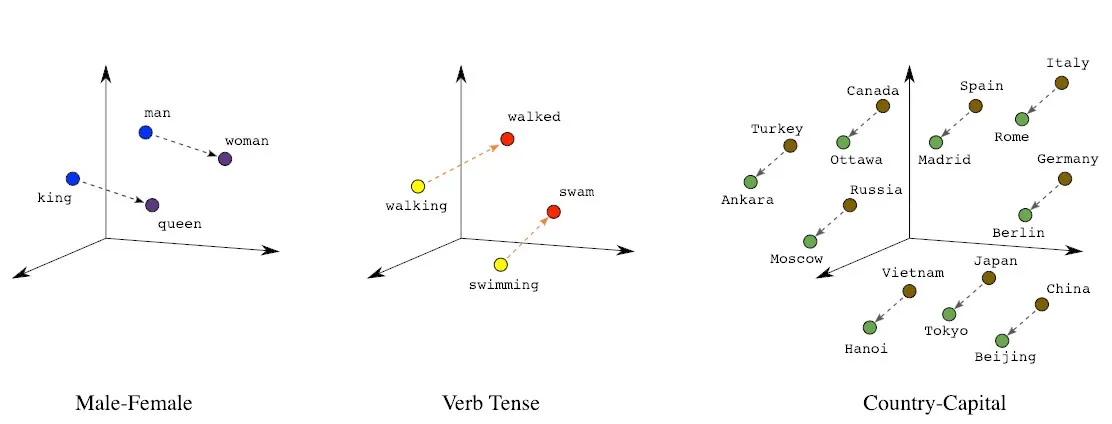
\includegraphics[width=1\textwidth]{../imgs/embeddings.png} % Ajusta la ruta y el ancho según necesites
    \caption{\tiny Además, vemos como estas representaciones permiten establecer relaciones  tareas de analogía }
    \label{miimagen}
\end{figure}
\end{frame}
\begin{frame}{Word2Vec - Visualización}
\begin{itemize}
\item Veamos ahora cómo se ve un embedding: \href{https://projector.tensorflow.org/}{TensorFlow Embedding Projector}
\end{itemize}
\end{frame}


\begin{frame}{W2V - Limitaciones}
\begin{itemize}
\item Si durante el entrenamiento no se ha encontrado un término, W2V no puede crear un vector para él y, en su lugar, asignará un vector aleatorio, lo cual no es óptimo. 
\item No tiene representaciones compartidas a nivel de subpalabras
\item Difícil de escalar a nuevos idiomas
\end{itemize}
\end{frame}

\begin{frame}{FastText}
\begin{itemize}
%\item Propuesto por Bojanowski et al (2016) https://arxiv.org/abs/1607.04606
\item Propuesto por \cite{bojanowski2016enriching}

\item A diferencia de W2V, incorpora información de subpalabras
\item Captura información de la estructura morfologica 
\item Cada palabra es representada como un conjunto de n-gramas a nivel del caracter

\end{itemize}

\end{frame}

\begin{frame}{FastText: Subwords}
    \centering
    \includegraphics[width=0.45\textwidth]{../imgs/fasttext-subwordspng.png}
    
    \vspace{1em} % Espacio entre imagen y texto

    {\footnotesize % O usa \scriptsize si lo querés más compacto
    \begin{itemize}
        \item Un \textbf{n-gram de caracteres} es un conjunto de caracteres co-ocurrentes dentro de una ventana.
        \item Una \textbf{bolsa de n-gramas} representa una palabra como la suma de sus n-gramas.
        \item Asume implícitamente que cada n-gram es igualmente importante independientemente del contexto, pero, en realidad, ese no es el caso porque no todos los n-gramas son un morfema.
    \end{itemize}
    }
\end{frame}

\begin{frame}
Recapitulemos: 
\begin{itemize}
\item Con lo que vimos hasta acá sabemos que existen al menos dos objetivos al entrenar un modelo de embeddings 
\begin{itemize}
\item Predecir una palabra dado su contexto
\item Predecir un contexto dado una palabra central
\end{itemize}
\item Tanto W2V como FastText generan Embeddings Estáticos, es decir, más allá de dónde aparezca la palabra, el vector será el mismo
\item Ambos utilizan una arquitectura similar que contiene una capa de entrada, una capa intermedia y una capa de salida. 
\item Entrenan en un gran corpus, ajustando pesos para que las palabras con contextos similares tengan vectores similares.
\end{itemize}

\end{frame}

\begin{frame}{Embeddings Contextuales}
\begin{itemize}
\item ELMo: Embeddings contextuales usando LSTM bidireccional
 \item Procesan una sequencia de derecha a izquierda y de izquierda a derecha
\item Capaz de extraer un embedding para cada palabra dependiendo de la posicion en la secuencia
\item Transformer y Attention: Permitieron procesar secuencias en paralelo y atender a palaras alejadas sin tener que pasar secuencialmente por cada token 
\end{itemize}
\end{frame}

\begin{frame}{ Modelos basados en Transformers}
\begin{itemize}
\item Generan embeddings contextuales.
\item La misma palabra puede tener diferentes representaciones según el contexto. 
\item Tienen una comprension mayor del concepto de ambiguedad y polisemia, ya que generan representaciones en funcion del contexto.
\item Son más potentes, aunque se alejan del concepto tradicional de embeddings fijos.
\item Modelos como \textbf{BERT} generan vectores a nivel del token, de la oración o del segmento y de la \textbf{posición}.
\end{itemize}
\end{frame}

%
%\begin{frame}{Tokenización en Transformers}
%En el caso de los Transformers, hacen uso de lo que se conoce como P
%
%\vspace{1em}
%
%  \textbf{Ejemplo:}  
%  \[
%    \underbrace{\detokenize{[CLS]}}_{\text{Token de inicio}} \quad
%    \underbrace{\detokenize{Un}}_{\text{Token 1}} \quad
%    \underbrace{\detokenize{ejem}}_{\text{Token 2}} \quad
%    \underbrace{\detokenize{plo}}_{\text{Token 3}} \quad
%    \underbrace{\detokenize{muy}}_{\text{Token 4}} \quad
%    \underbrace{\detokenize{interesante}}_{\text{Token 5}} \quad
%    \underbrace{\detokenize{[SEP]}}_{\text{Token de fin}}
%  \]
%  
%  \vspace{0.3cm}
%  
%  \footnotesize
%  En este ejemplo, el modelo tokeniza la oración descomponiendo las palabras en subunidades, lo que permite obtener embeddings a nivel de token. Estos se pueden agrupar para obtener representaciones de palabra, oración o incluso del documento completo, ofreciendo una mayor riqueza contextual frente a los embeddings fijos de Word2Vec.
%\end{frame}

\begin{frame}
\begin{figure}{BERT Embeddings}
    \centering
    \includegraphics[width=1\textwidth]{../imgs/contextualembeddings.png} % Ajusta la ruta y el ancho según necesites
    \caption{\tiny Aquí podemos ver como esta serie de arquitecturas generan embeddings para diferentes niveles de representación}
    \label{miimagen}
\end{figure}
\end{frame}

%
%\begin{frame}{Comparación: Word2Vec vs. Embeddings en Transformers}
%  \begin{columns}[T]
%    \column{0.48\textwidth}
%      \textbf{Word2Vec}
%      \begin{itemize}
%        \item Representa palabras completas.
%        \item Cada palabra tiene un vector fijo.
%        \item No descompone palabras en subunidades.
%        \item Embeddings estáticos (sin variación según el contexto).
%      \end{itemize}
%      
%    \column{0.48\textwidth}
%      \textbf{Embeddings en Transformers}
%      \begin{itemize}
%        \item \textbf{Tokenización subpalabra}: Los tokens pueden ser partes de palabras (ej.: ``ejem'', ``plo'').
%        \item \textbf{Contextualizados}: Cada token obtiene un vector según su contexto.
%        \item \textbf{Múltiples niveles}: Se pueden extraer representaciones a nivel de:
%          \begin{itemize}
%            \item Token
%            \item Palabra (agrupando tokens)
%            \item Oración
%            \item Documento
%          \end{itemize}
%      \end{itemize}
%  \end{columns}
%\end{frame}

\begin{frame}{Contextual vs. Estáticos}
  \begin{columns}[T]
    \column{0.48\textwidth}
      \textbf{Word2Vec / FastText (Estáticos)}
      \begin{itemize}
        \item Una palabra = un vector, fijo y sin variación por contexto.
        \item Arquitectura simple, \textit{feed-forward} (Skip-gram / CBOW).
        \item Buen rendimiento en tareas básicas, muy eficientes.
        \item Limitación: no distinguen significados múltiples de la misma palabra.
      \end{itemize}
    \column{0.48\textwidth}
      \textbf{Embeddings en Transformers (Contextuales)}
      \begin{itemize}
        \item Cada palabra (o subpalabra) obtiene un vector distinto según el contexto.
        \item Basados en \textbf{self-attention}, permiten paralelización.
        \item Mayor capacidad de capturar matices semánticos.
        \item \textit{Ejemplo}: BERT, GPT, etc. con potencial para tareas complejas.
      \end{itemize}
  \end{columns}
\end{frame}
%------------------

%------------------
\begin{frame}{Arquitectura y Entrenamiento}
  \begin{itemize}
    \item \textbf{Word2Vec / FastText}:
      \begin{itemize}
        \item Modelo \textbf{feed-forward} de 2 capas.
        \item Objetivo de entrenamiento: predecir el contexto (\textit{Skip-gram}) o la palabra central (\textit{CBOW}).
        \item \textit{Subpalabras en FastText}, pero siguen siendo embeddings estáticos.
      \end{itemize}

    \vspace{0.5em}
    \item \textbf{Transformers}:
      \begin{itemize}
        \item \textbf{Autoatención} (\textit{self-attention}) en cada capa, eliminando la recurrencia.
        \item Objetivos de entrenamiento diferentes:
          \begin{itemize}
            \item BERT: \textit{Masked Language Modeling} (MLM).
            \item GPT: \textit{Causal Language Modeling} (predicción izquierda a derecha).
          \end{itemize}
        \item Embeddings \textbf{posicionales} para codificar orden de tokens.
      \end{itemize}
  \end{itemize}
\end{frame}
%------------------

%------------------
\begin{frame}{Ejemplo de Polisemia: \textit{Banco}}
  \textbf{Ilustración de embeddings estáticos vs. contextuales:}\\[6pt]
  \begin{columns}[T]
    \column{0.5\textwidth}
      \textbf{Oraciones:}
      \begin{itemize}
        \item ``Me senté en el \textbf{banco} de la plaza.''
        \item ``Fui al \textbf{banco} a sacar dinero.''
      \end{itemize}
    \column{0.5\textwidth}
      \textbf{Comparación:}
      \begin{itemize}
        \item \textbf{Word2Vec}: 
          \begin{itemize}
            \item Mismo vector para ``banco'' en ambos casos.
          \end{itemize}
        \item \textbf{Transformers (ej. BERT)}:
          \begin{itemize}
            \item \textbf{Embeddings diferentes} para ``banco'' (mueble vs. entidad financiera).
            \item Captura el \textbf{contexto} alrededor.
          \end{itemize}
      \end{itemize}
  \end{columns}
  \vspace{0.5em}
  \textit{Resultado:} Los modelos contextuales permiten desambiguar sentidos que un embedding estático no distingue.
\end{frame}
%------------------

%------------------
\begin{frame}{Conclusiones y Aplicaciones}
  \begin{itemize}
    \item \textbf{Word2Vec / FastText}:
      \begin{itemize}
        \item Fáciles de entrenar, muy rápidos y buenos para tareas simples o recursos limitados.
        \item Representaciones \textbf{estáticas} no diferencian polisemia.
      \end{itemize}
    \item \textbf{Transformers (LLMs)}:
      \begin{itemize}
        \item Modelos \textbf{profundos y contextuales}, apropiados para problemas más complejos (QA, NER, semántica avanzada).
        \item Requieren más \textbf{recursos de cómputo} y mayor complejidad de implementación.
      \end{itemize}
  \end{itemize}
\end{frame}


\section{Bibliografía}
\begin{frame}[allowframebreaks]{Bibliografía}
\bibliography{../biblio-y-paquetes/bibliogeneral}
\bibliographystyle{../biblio-y-paquetes/apalike-es}
\end{frame}

\end{document}
